% bei Standalone in documentclass noch:
% \RequirePackage{luatex85}

\documentclass[captions=tableheading, titlepage= firstiscover, parskip = half , bibliography=totoc]{scrartcl}
%paper = a5 für andere optinen
% titlepage= firstiscover
% bibliography=totoc für bibdateien
% parskip=half  Veränderung um Absätze zu verbessern

\usepackage{scrhack} % nach \documentclass
\usepackage[aux]{rerunfilecheck}
\usepackage{polyglossia}
\usepackage[style=numeric, backend=biber]{biblatex} % mit [style = alphabetic oder numeric] nach polyglossia
\addbibresource{lit.bib}
\setmainlanguage{german}

\usepackage[autostyle]{csquotes}
\usepackage{amsmath} % unverzichtbare Mathe-Befehle
\usepackage{amssymb} % viele Mathe-Symbole
\usepackage{mathtools} % Erweiterungen für amsmath
\usepackage{fontspec} % nach amssymb
% muss ins document: \usefonttheme{professionalfonts} % für Beamer Präsentationen
\usepackage{longtable}

\usepackage[
math-style=ISO,    % \
bold-style=ISO,    % |
sans-style=italic, % | ISO-Standard folgen
nabla=upright,     % |
partial=upright,   % /
]{unicode-math} % "Does exactly what it says on the tin."
\setmathfont{Latin Modern Math}
% \setmathfont{Tex Gyre Pagella Math} % alternativ

\usepackage[
% die folgenden 3 nur einschalten bei documenten
locale=DE,
separate-uncertainty=true, % Immer Fehler mit ±
per-mode=symbol-or-fraction, % m/s im Text, sonst \frac
]{siunitx}

% alternativ:
% per-mode=reciprocal, % m s^{-1}
% output-decimal-marker=., % . statt , für Dezimalzahlen

\usepackage[
version=4,
math-greek=default,
text-greek=default,
]{mhchem}

\usepackage[section, below]{placeins}
\usepackage{caption} % Captions schöner machen
\usepackage{graphicx}
\usepackage{grffile}
\usepackage{subcaption}

% \usepackage{showframe} Wenn man die Ramen sehen will

\usepackage{float}
\floatplacement{figure}{htbp}
\floatplacement{table}{htbp}

\usepackage{mhchem} %chemische Symbole Beispiel: \ce{^{227}_{90}Th+}


\usepackage{booktabs}

 \usepackage{microtype}
 \usepackage{xfrac}

 \usepackage{expl3}
 \usepackage{xparse}

 % \ExplSyntaxOn
 % \NewDocumentComman \I {}  %Befehl\I definieren, keine Argumente
 % {
 %    \symup{i}              %Ergebnis von \I
 % }
 % \ExplSyntaxOff

 \usepackage{pdflscape}
 \usepackage{mleftright}

 % Mit dem mathtools-Befehl \DeclarePairedDelimiter können Befehle erzeugen werden,
 % die Symbole um Ausdrücke setzen.
 % \DeclarePairedDelimiter{\abs}{\lvert}{\rvert}
 % \DeclarePairedDelimiter{\norm}{\lVert}{\rVert}
 % in Mathe:
 %\abs{x} \abs*{\frac{1}{x}}
 %\norm{\symbf{y}}

 % Für Physik IV und Quantenmechanik
 \DeclarePairedDelimiter{\bra}{\langle}{\rvert}
 \DeclarePairedDelimiter{\ket}{\lvert}{\rangle}
 % <name> <#arguments> <left> <right> <body>
 \DeclarePairedDelimiterX{\braket}[2]{\langle}{\rangle}{
 #1 \delimsize| #2
 }

\setlength{\delimitershortfall}{-1sp}

 \usepackage{tikz}
 \usepackage{tikz-feynman}

 \usepackage{csvsimple}
 % Tabellen mit \csvautobooktabular{"file"}
 % muss in table umgebung gesetzt werden


% \multicolumn{#Spalten}{Ausrichtung}{Inhalt}

\usepackage{hyperref}
\usepackage{bookmark}
\usepackage[shortcuts]{extdash} %nach hyperref, bookmark

\newcommand{\ua}[1]{_\symup{#1}}
\newcommand{\su}[1]{\symup{#1}}


\begin{document}

\section{Auswertung}

\subsection{Messung der Zeitkonstanten mit einer Entladekurve}

In dem ersten Teil des Versuches wird mit dem Oszilloskop die Entladekurve des
sich im RC-Kreis befindenden Kondensators betrachtet. Dem in Abbildung \ref{fig:thermodruck}
zu sehenden Thermodruck werden dabei 13 Wertepaare entnommen und in den Graphen
(Abbildung \ref{fig:Messunga}) eingetragen. Mithilfe einer linearen Regression nach
Formel \eqref{eqn:FitMessungA} kann dann die Steigung ermittelt werden, deren
Kehrwert im Betrag der Zeitkonstante $RC$ entspricht.

\begin{align}
  \label{eqn:FitMessungA}
  ln \left( U\ua{C} \right) &= m \cdot t + b \\
  m    &= -\frac{1}{RC}
\end{align}

\begin{table}
  \centering
  \caption{Entnommene Wertepaare für die Spannungsamplituden zu verschiedenen
          Zeitpunkten des Entladevorgangs}
  \label{tab:MessungA}
  \begin{tabular}{c c || c c}
    \toprule $t \,\, in \,\, \su{ms}$ & $U\ua{C} \,\, in \,\, \su{V}$ &
             $t \,\, in \,\, \su{ms}$ & $U\ua{C} \,\, in \,\, \su{V}$ \\
    \midrule
    0.00 & 12.4 & 1.75 & 3.4 \\
    0.25 & 10   & 2.00 & 2.8 \\
    0.50 &  8.2 & 2.25 & 2.4 \\
    0.75 &  6.6 & 2.50 & 2   \\
    1.00 &  5.8 & 2.75 & 1.8 \\
    1.25 &  4.6 & 3.00 & 1.6 \\
    1.50 &  4   & -    & -   \\
    \bottomrule
  \end{tabular}
\end{table}

Mithilfe der linearen Regression ergibt sich dabei für die Zeitkonstante $RC$ ein
Wert von $RC = (0.00146 \pm 0.00003) \, \su{s}$.

\begin{figure}
  \centering
  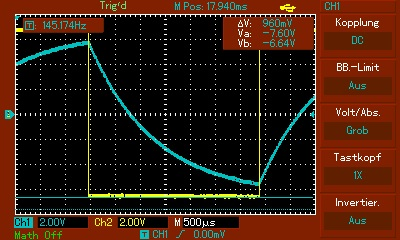
\includegraphics[width = 12 cm]{Sternchen.jpg}
  \caption{Thermodruck der in Messung x.x betrachteten Entladekurve }
  \label{fig:thermodruck}
\end{figure}

\begin{figure}
  \centering
  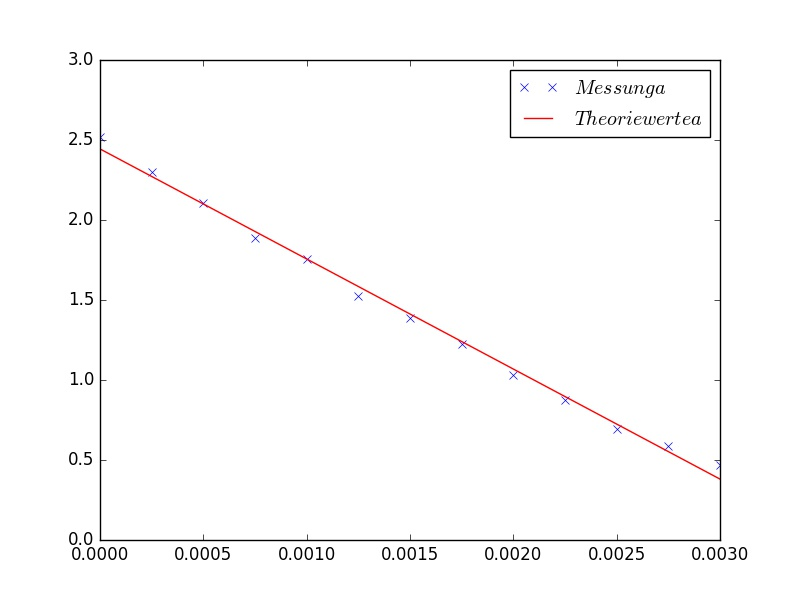
\includegraphics[width = 12 cm]{Messunga.jpg}
  \caption{gemessene Werte für $U\ua{C}$ aufgetragen gegen die Zeit $t$}
  \label{fig:Messunga}
\end{figure}

%Eingügen der Grafik mit den eingetragenenen Werten

\newpage

\subsection{Bestimmung der Zeitkonstanten über Messung der zeitabhängigen Spannungsamplitude}

In der zweiten Messung des Versuches wurde mithilfe des Oszilloskopes die Spannungsamplitude
an dem Kondensator in Abhängigkeit der Frequenz gemessen. Die gemessenen Werte
werden logarythmisch in dem Graphen aufgetragen und mithilfe eines Regressionskurve
nach Formel \eqref{eqn:FitMessungB} kann dann die Zeitkonstante RC bestimmt werden,
die in Formel \eqref{eqn:FitMessungB} der Konstante a entspricht.

\begin{equation}
  A(\nu) = \frac{1}{ \sqrt{ 1 + ( 2 \cdot \pi \cdot x )^2 \cdot a^2}}
  \label{eqn:FitMessungB}
\end{equation}

Aus der Abbildung \ref{fig:Messungb} ergibt sich somit mit der Regressionskurve
für die Zeitkonstante folgender Wert:

\begin{equation}
  RC = a = (0.00130 \pm 0.00002) \, \su{s} .
\end{equation}

\begin{figure}
  \centering
  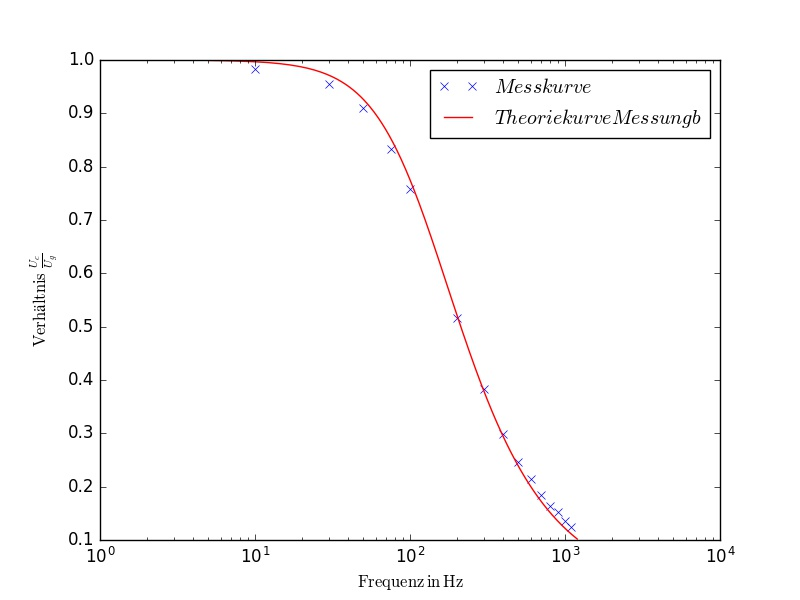
\includegraphics[width = 12 cm]{Messungb.jpg}
  \caption{Verhältnis der gemessenen Spannungsamplituden $U\ua{C}$ und der Ausgangsspannung $U\ua{0}$
           aus Tabelle ?? aufgetragen gegen die Frequenz $\nu$}
  \label{fig:Messungb}
\end{figure}



















\end{document}
